\subsection{Gaussian Splatting}
Przy pomocy biblioteki \textit{gsplat}\cite{ye2024gsplatopensourcelibrarygaussian} zawierającej implementację \textit{Gaussian Splatting} w Pythonie wykonane zostały eksperymenty polegające na uruchomeniu algorytmu dla różnych wartości hiperparametrów w celu znalezienia wartości które prowadzą do jak najbardziej optymalnego procesu trenowania w kontekście czasu trwania i wykorzystania pamięci. 

Na wejściu algorytmu podawana jest chmura punktów, która jest bazą do dalszego dzielenia i powstawania gaussianów, a ich parametry: pozycja, kolor, skala i rotacja są optymalizowane przy pomocy metody spadku wzdłuż gradientu. Metryki przyjęte do oceny jakości to \textbf{SSIM} (Structural Similarity Index Measure), \textbf{PSNR} (Peak Signal-to-Noise Ratio) oraz \textbf{LPIPS} (Learned Perceptual Image Patch Similarity).

Wykonane eksperymenty pokazały, że najważniejsze parametry dla przebiegu procesu to: 
\begin{enumerate}
    \item liczba Gaussianów: w przypadku scen urbanistycznych w celu oddania odpowieniej szczegółowości potrzebne jest kilka milionów Gaussianów,
    \item strategia i częstość adaptacji: określają w jaki sposób oraz jak często dodawane i usuwane są Gaussiany, 
    \item liczba iteracji: zwykle im dłużej trenowana jest scena tym wyniki są lepsze, jednak zależy to również od przyjętej strategii. Liczba ta wpływa bezpośrednio na czas trenowania, powinna wynieść nie mniej niż kilkanaście tysięcy,
    \item stopień zmiennych harmonicznych: wyrażają one kolor, im większy stopień tym lepsza jakość sceny, ale też zwiększone zużycie pamięci i wydłużony czas trenowania. 
\end{enumerate}

Ilustracje \ref{fig:sks_gs}, \ref{fig:c5_gs} oraz \ref{fig:c7_gs} przedstawiają przykładowe wizualizacje (od lewej do prawej: prawdziwe zdjęcie i widok modelu), a tabela \ref{table:tab_gs_res} zawiera wybrane wielkości dla scen testowych. Renderowania zostały wykonane przy pomocy biblioteki \textit{nerfview} która również służy do wizualizacji splatów.

\begin{figure}[!h]
    \centering
    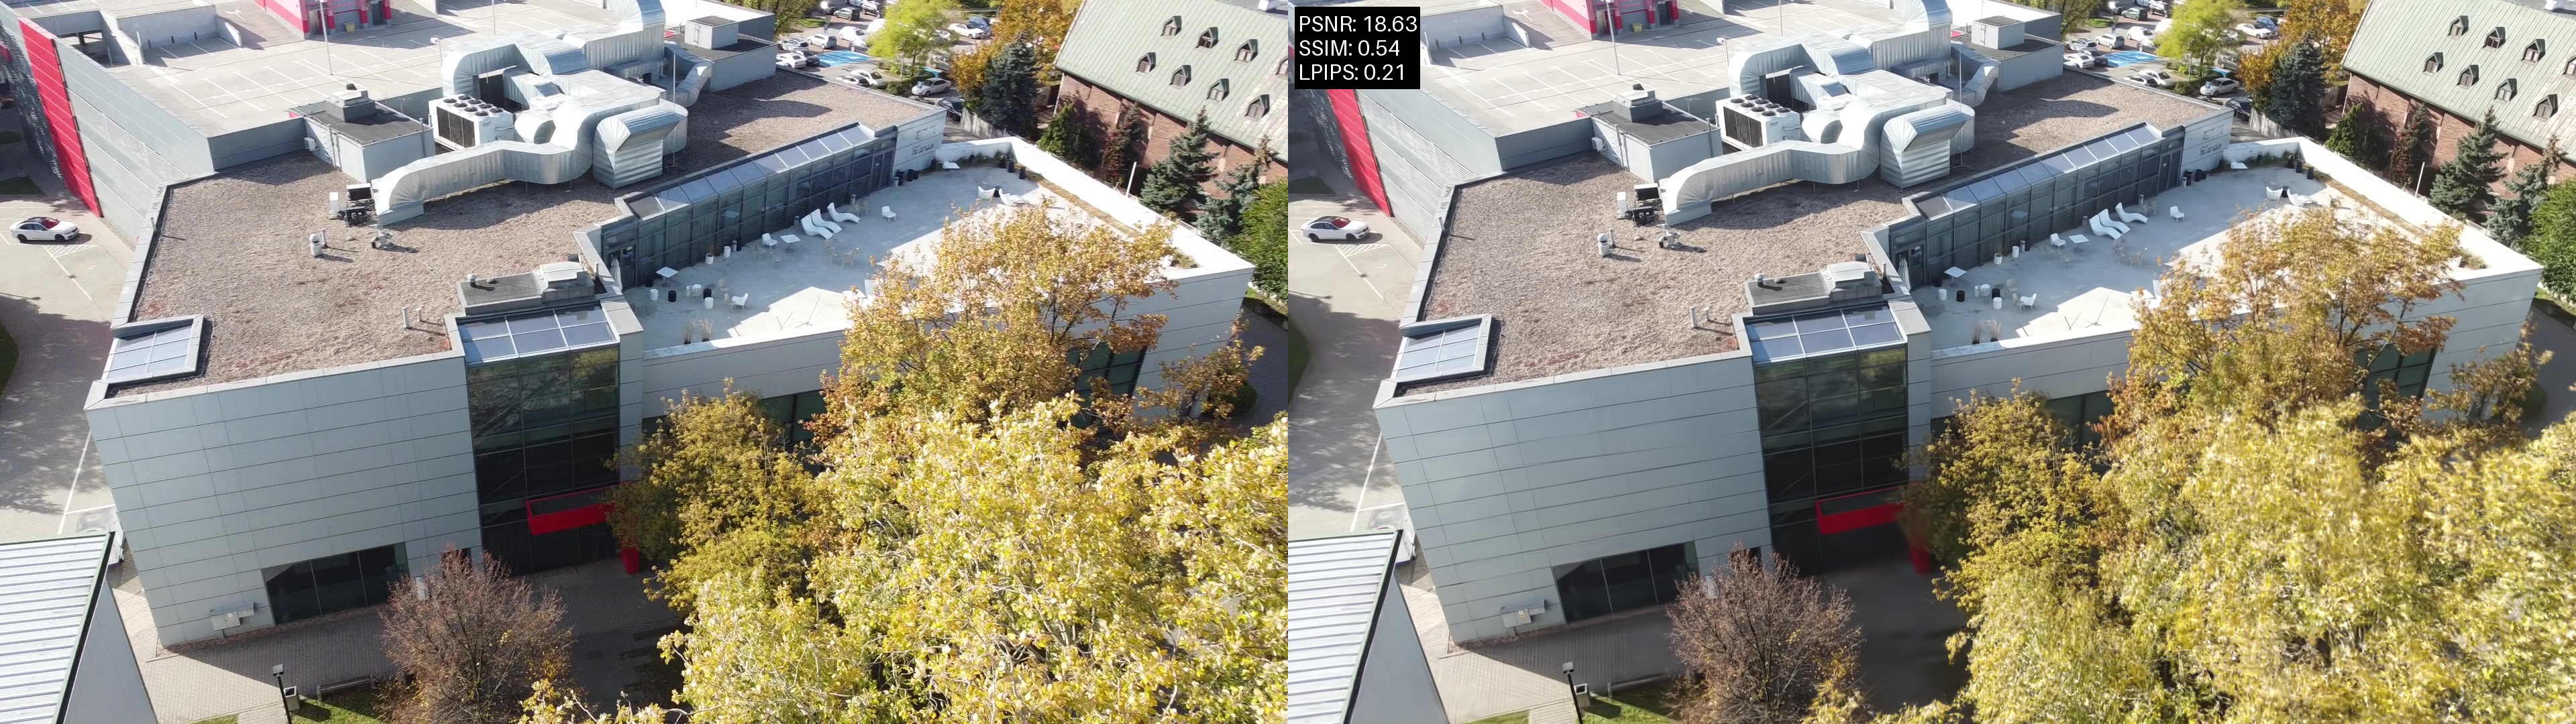
\includegraphics[width=1.0\linewidth]{images/sks_viper_0008.png}
    \caption{Scena SKS}
    \label{fig:sks_gs}
\end{figure}

\begin{figure}[!h]
    \centering
    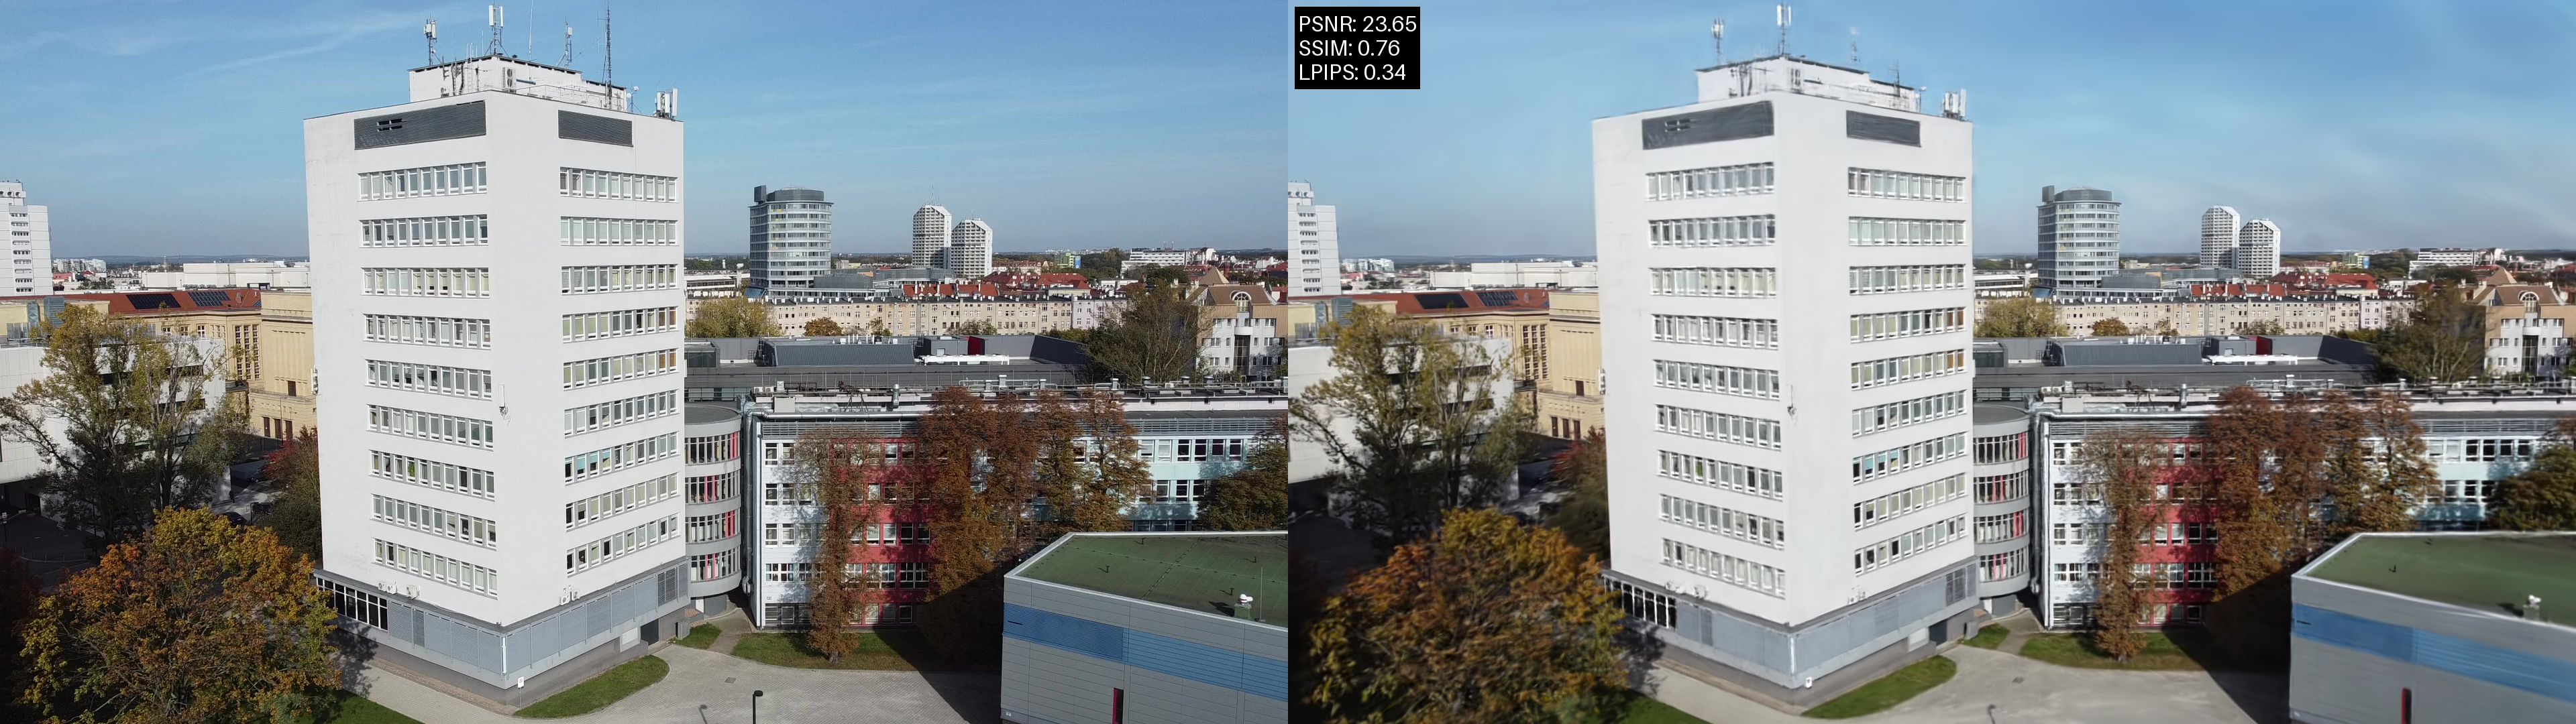
\includegraphics[width=1.0\linewidth]{images/c5_dinosaur_0001.png}
    \caption{Scena C5}
    \label{fig:c5_gs}
\end{figure}

\begin{figure}[!h]
    \centering
    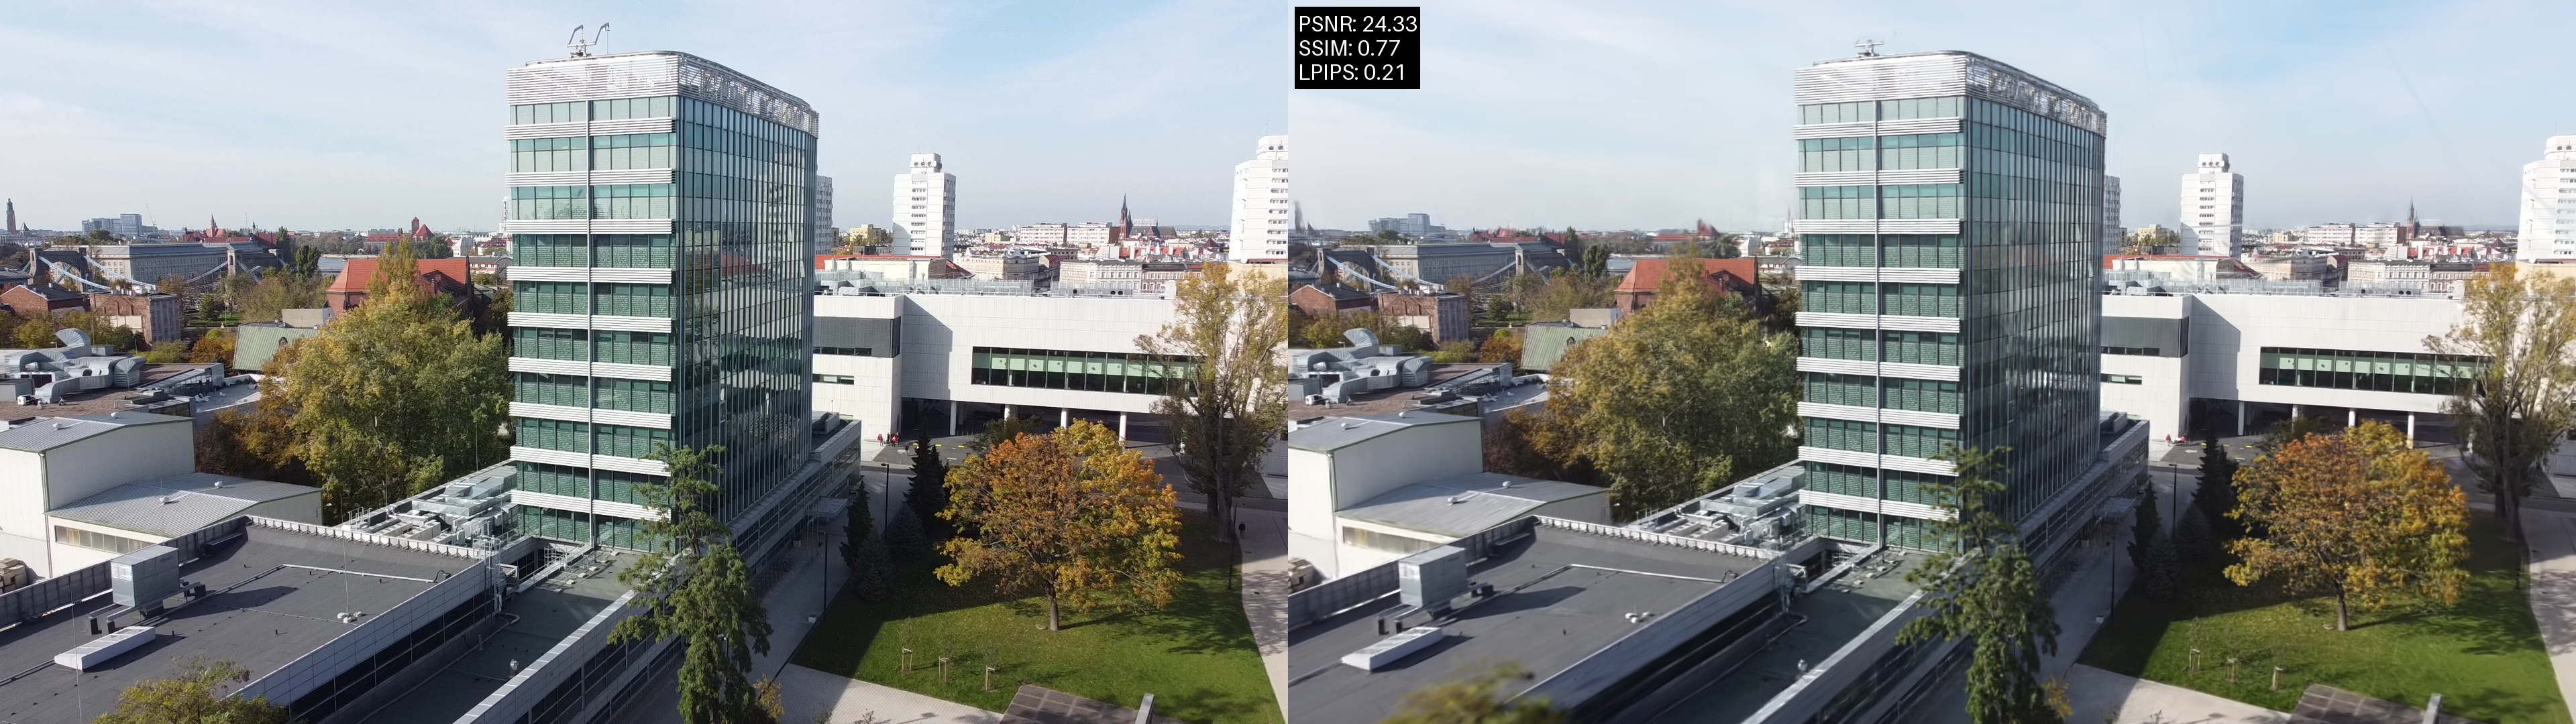
\includegraphics[width=1.0\linewidth]{images/c7_gepard_0006.png}
    \caption{Scena C7}
    \label{fig:c7_gs}
\end{figure}

\begin{table}[!h]
    \centering
    \begin{tabular}{|c|c|c|c|c|c|c|}
    \hline
    scena & PSNR & SSIM & LPIPS & liczba gaussianów & czas trenowania & pamięć pliku (MB) \\
    \hline 
    SKS & 22.03 & 0.71 & 0.25 & 2,937,549 & 2h53m & 661 \\
    \hline 
    C5 & 21.98 & 0.71 & 0.26 & 4,564,464 & 10h40m & 675 \\
    \hline 
    C7 & 22.63 & 0.72 & 0.29 & 3,000,000 & 15h15m & 675 \\
    \hline
    \end{tabular}
\caption{Całościowe metryki dla testowych scen. Otrzymane wartości PSNR, SSIM oraz LPIPS zwykle świadczą o dobrej jakości scenie, która oddaje wystarczające szczegóły i wygładzone artefakty.}
\label{table:tab_gs_res}
\end{table}